\section{Selection Criteria}
\label{sec:MissionSites:SelectionCriteria}
Mission sites were required before determining environmental constraints pertaining to available solar radiation on the Martian surface. These sites were selected based on the following criteria:

\begin{itemize}
    \item The location is of scientific interest, supported by past or ongoing research.
    \item The terrain features complex morphologies so that scenarios with inclined solar array surfaces may be simulated from which the rover's active suspension system may also be evaluated.
    \item Landing sites for the location have been proposed in preceedings such as with the \ac{MSL} Landing Site Workshops in \citeother{MSLLandingSites}. Such proposals suggest technical feasibility in landing a rover for the proposed locations.
    \item \ac{HiRISE} \ac{DTM} are available near the \ac{ROI} so that 3D environment models may be loaded on the mission simulation platform.
    \item The planetary latitude is close to that of the \ac{MER} Opportuniy mission in order to enable future comparative analysis of simulation results with 14 years worth of \ac{MER} power budget data. This target planetary latitude is approximately \SI{2}{\degree}S.
    \item The planetary latitude is close to that of the \ac{VL1} and \ac{VL2} missions in order to more closely align with the environment conditions from which the power and energy prediction models were built. This target planetary latitude is between \SI{22}{\degree}N and \SI{48}{\degree}N.
\end{itemize}

The latter two criteria being mutually exclusive, two locations were selected: Iani Chaos and Ismenius Cavus. Conducting mission scenario simulations for both locations also ensured that a wider range of seasonal driven solar radiation constraints were explored with respect to differences in planetary latitude.

\clearpage
\section{Iani Chaos}
\label{sec:MissionSites:IaniChaos}
Iani Chaos is centered at approximately \SI{342}{\degree}E, \SI{2}{\degree}S, it is scientific interest due its long-lived, but likely episodic, fluvial activity \citeother{Warner2011}. In particular, hematite- and sulfite-rich light-toned layered deposits suggest past shallow water and groundwater depositional environment \citeother{Glotch2007}. Figure \ref{fig:mission-site-iani-chaos} shows the distribution of these deposits in region covering \SI{9}{\degree}S – \SI{4}{\degree}N latitude and \SI{328}{\degree} – \SI{348}{\degree}E longitude. Furthermore, ``topography, the observed geomorphology, and measured fracture patterns suggest that the interchaos basins formed as a result of subsurface volume loss and collapse of the crust, likely owing to effusion of groundwater to the surface'' \citeother{Warner2011}. Iani Chaos is a ``clear link to the past presence of surface and subsurface water, making the site of prime astro-biological interest.'' \citeother{Glotch2006}

\begin{figure}[h]
  \centering
  \hypersetup{linkcolor=captionTextColor}
  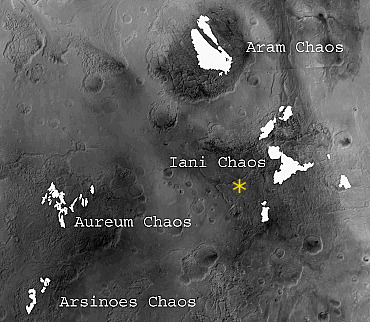
\includegraphics[width=0.5\linewidth]{sections/mission-sites/images/iani-chaos-deposits.png}\\
  \caption[Map of light‐toned deposits in chaotic terrains in Margaritifer Terra overlaid on a \ac{MOC} \ac{WA} mosaic]
          {Map of light‐toned deposits in chaotic terrains in Margaritifer Terra overlaid on a \ac{MOC} \ac{WA} mosaic. The mapped region covers \SI{9}{\degree}S – \SI{4}{\degree}N latitude and \SI{328}{\degree} – \SI{348}{\degree}E longitude. Taken from \citeother{Glotch2007}. The yellow asterisk indicates the \ac{HiRISE} \ac{DTM} location in Western Iani Chaos which was used for mission scenario simulation.}
  \label{fig:mission-site-iani-chaos}
\end{figure}

Iani Chaos is ``among the most geomorphologically complex chaotic terrains.'' From  \citeother{Warner2011}, it's morphology has been defined by:

\begin{itemize}
    \item Multiple, 1 to \SI{2}{\kilo\meter} deep basins.
    \item Flat‐topped, fractured plateaus that are remnants of highland terrain.
    \item Knobby, fractured remnants of highland terrain.
    \item Plateaus with a knobby surface morphology.
    \item Interchaos grooved terrain.
    \item \ac{ILD}.
    \item Mantling material.
\end{itemize}

Figure \ref{fig:sub:western-iani-chaos-dtm} shows a section of the \ac{DTM} of Western Iani Chaos which was loaded on the rover's mission simulation plaform. The topography of the area is shown in Figure \ref{fig:sub:western-iani-chaos-dtm-altimetry}.

\vspace{0.5cm}

\begin{figure}[h]
\captionsetup[subfigure]{justification=centering}
\vspace{-2ex}
	\centering
    %% setup sizes
    \setlength{\subfigureWidth}{0.50\textwidth}
    \setlength{\graphicsHeight}{130mm}
    %% kill hyper-link highlighting
    \hypersetup{hidelinks=true}%
    %% the figures
    \begin{subfigure}[t]{\subfigureWidth}
        \centering
        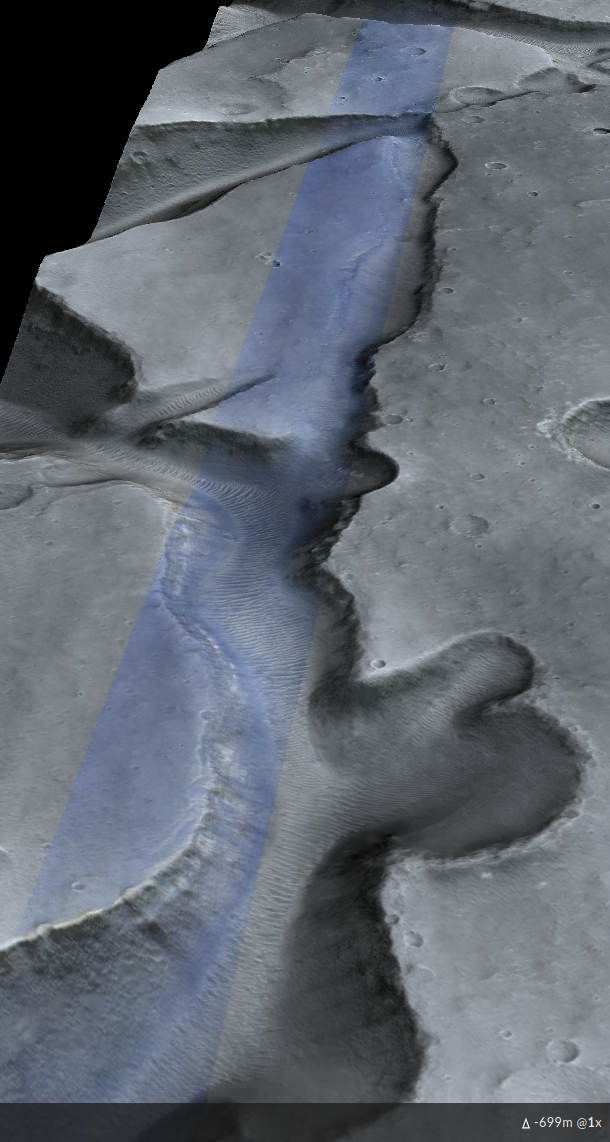
\includegraphics[height=\graphicsHeight]{sections/mission-sites/images/western-iani-chaos-dtm.png}
        \subcaption{\ac{DTM}}
        \label{fig:sub:western-iani-chaos-dtm}
    \end{subfigure}\hfill
    \begin{subfigure}[t]{\subfigureWidth}
        \centering
        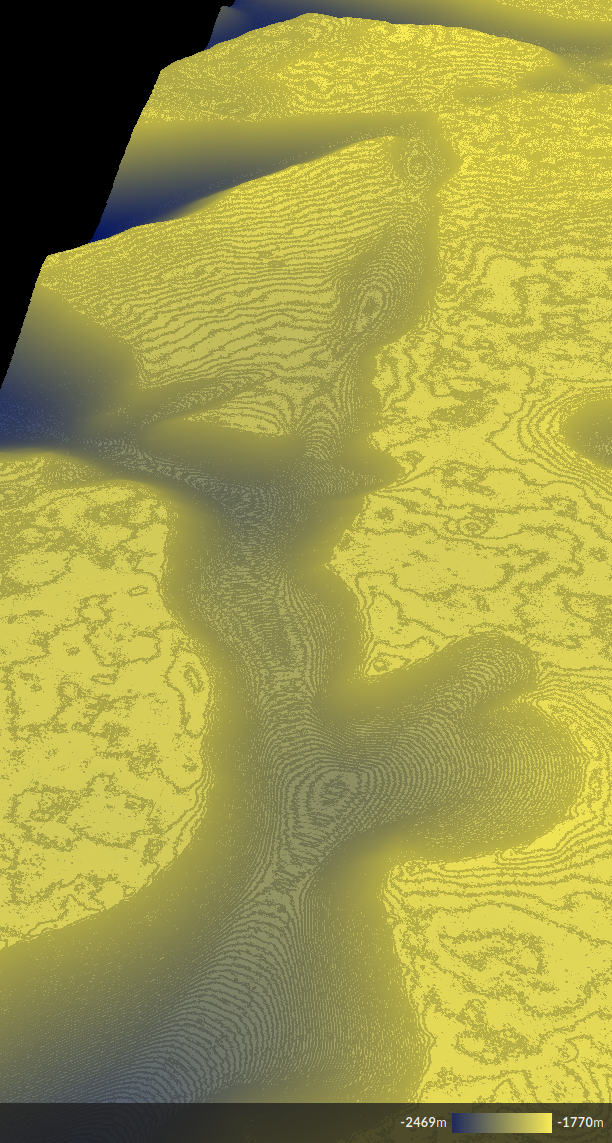
\includegraphics[height=\graphicsHeight]{sections/mission-sites/images/western-iani-chaos-dtm-altimetry.png}
  		\subcaption{Topography}
		\label{fig:sub:western-iani-chaos-dtm-altimetry}
	\end{subfigure}\\[0.8ex]
    \caption[Western Iani Chaos \ac{HiRISE} \ac{DTM}]
            {Western Iani Chaos \ac{HiRISE} \ac{DTM}, taken from \citeother{AreoBrowser}. Image: \ac{NASA}/\ac{JPL}/University of Arizona.}
    \label{fig:western-iani-chaos}
\vspace{-2ex}
\end{figure}

\clearpage

\section{Ismenius Cavus}
\label{sec:MissionSites:IsmeniusCavus}
Ismenius Cavus is located at \SI{33.5}{\degree}N, \SI{17}{\degree}E, with elevations ranging from \SI{-3.5}{\kilo\meter} and \SI{-1.5}{\kilo\meter}. It is a basin where several fluvial valleys converge and is located ``at the junction between current mid-latitude ice deposits and low latitude clay minerals'', hosting science and resource regions of interest ``with both present ice and past lake sediments with clay minerals'' \citeother{Dehouck2010} \citeother{Dehouck2015}. Geologic context for this mission site area is provided with Figure \ref{fig:mission-site-ismenius-cavus}.

\begin{figure}[h]
  \centering
  \hypersetup{linkcolor=captionTextColor}
  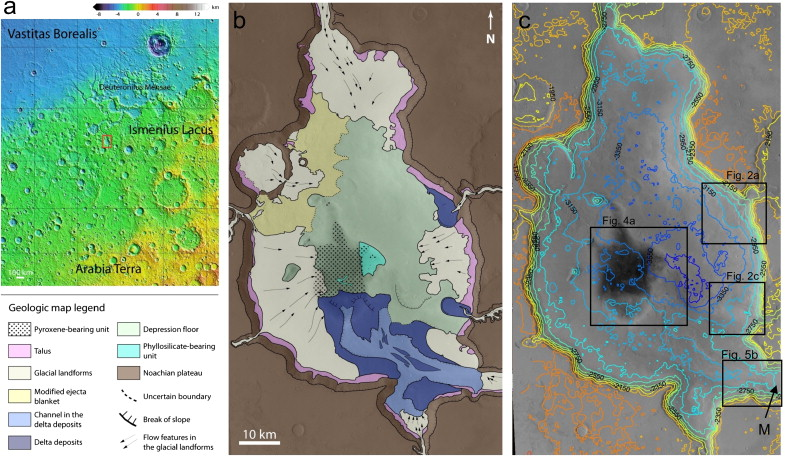
\includegraphics[width=0.8\linewidth]{sections/mission-sites/images/ismenius-cavus.png}\\
  \caption[Geologic context for Ismenius Cavus mission site area]
          {Geologic context of the mission site area, taken from \citeother{Dehouck2010}. Location shown on a \ac{MOLA} reference map (a) and a geologic map of Ismenius Cavus (b). The yellow asterisk indicates the \ac{HiRISE} \ac{DTM} location which was used for mission scenario simulation.}
  \label{fig:mission-site-ismenius-cavus}
\end{figure}

% https://www.uahirise.org/dtm/dtm.php?ID=ESP_052945_2150

Supported science of interest are taken from \citeother{Dehouck2015}:
\begin{itemize}
    \item Potential for past habitability.
    \item Potential for organic matter with surface exposure.
    \item Noachian/Hesperian rocks with trapped atmospheric gases.
    \item High likelohood of surface-atmosphere exchange.
    \item Amazonian subsurface or high-latitude ice or sediment.
    \item Range of martian geologic time; datable surfaces.
    \item Evidence of aqueous processes.
    \item Potential for interpreting relative ages.
    \item Near-surface ice, glacial or permafrost.
    \item Noachian or pre-Noachian bedrock units.
    \item Diversity of aeolian sediments and/or landforms.
\end{itemize}

Supported resources of interest are also presented in \citeother{Dehouck2015} with clay minerals and water ice being two main resources for water. Furthermore, there is a potential for metal/silicon. These resources are located no more than \SI{3}{\meter} below the surface. Mobile material resources for construction purposes also exist.

Figure \ref{fig:sub:ismenius-cavus-dtm} shows a section of the \ac{DTM} which was loaded on the rover's mission simulation plaform. It features an exit breach in a well-preserved crater. The topography of the area is shown in Figure \ref{fig:sub:western-iani-chaos-dtm-altimetry}.
\vspace{0.5cm}

\begin{figure}[h]
\captionsetup[subfigure]{justification=centering}
\vspace{-2ex}
	\centering
    %% setup sizes
    \setlength{\subfigureWidth}{0.50\textwidth}
    \setlength{\graphicsHeight}{100mm}
    %% kill hyper-link highlighting
    \hypersetup{hidelinks=true}%
    %% the figures
    \begin{subfigure}[t]{\subfigureWidth}
        \centering
        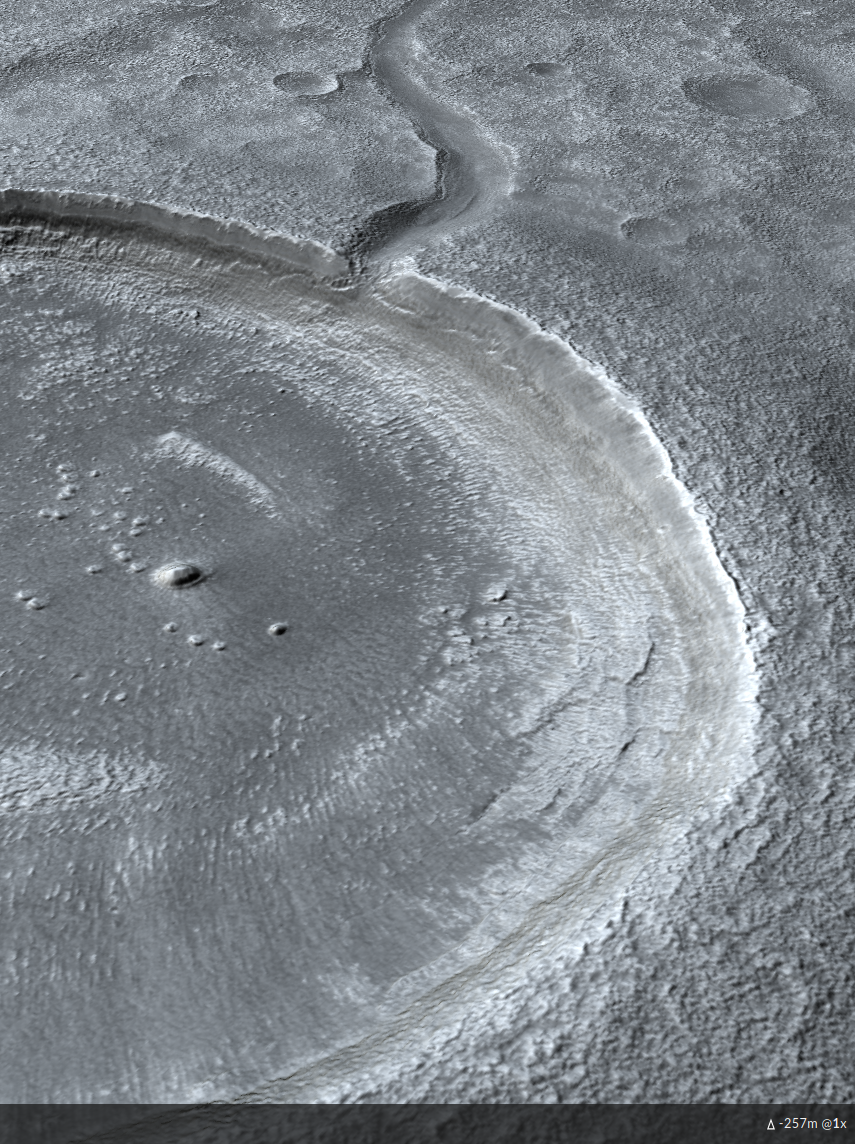
\includegraphics[height=\graphicsHeight]{sections/mission-sites/images/ismenius-cavus-dtm.png}
        \subcaption{\ac{DTM}}
        \label{fig:sub:ismenius-cavus-dtm}
    \end{subfigure}\hfill
    \begin{subfigure}[t]{\subfigureWidth}
        \centering
        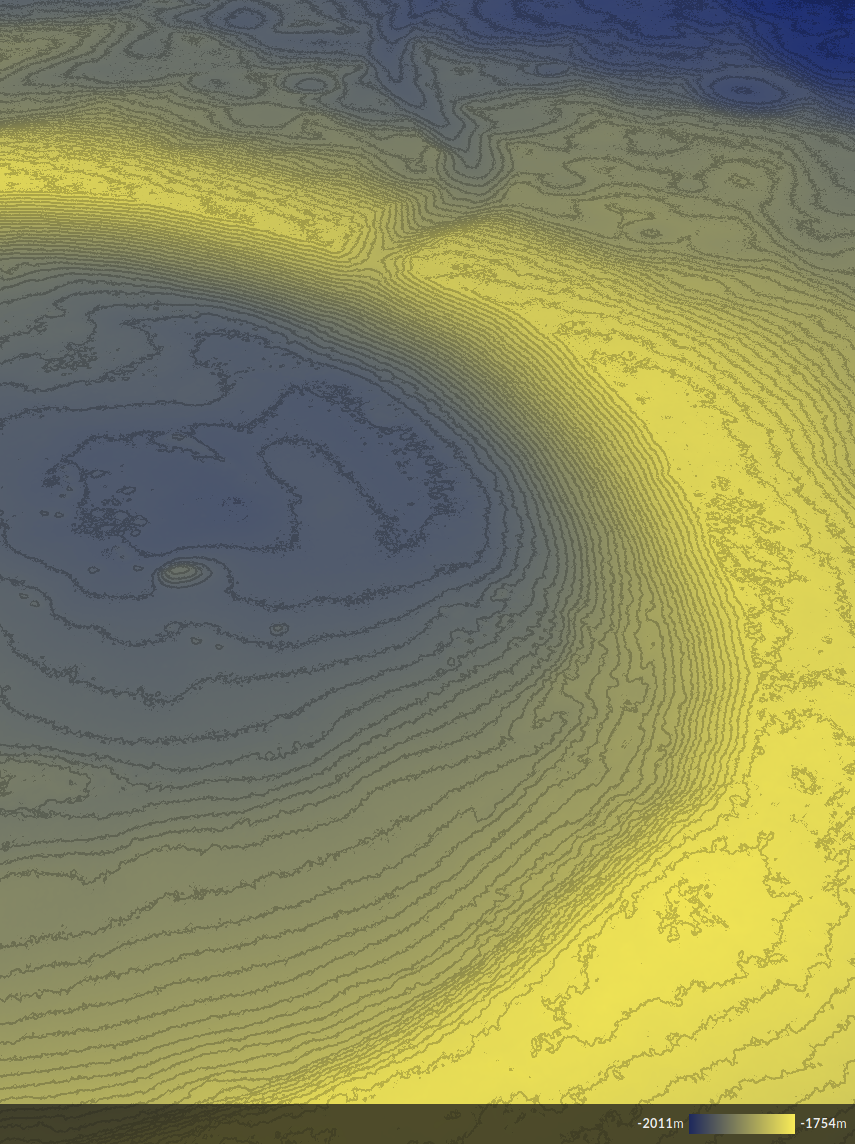
\includegraphics[height=\graphicsHeight]{sections/mission-sites/images/ismenius-cavus-dtm-altimetry.png}
  		\subcaption{Topography}
		\label{fig:sub:ismenius-cavus-dtm-altimetry}
	\end{subfigure}\\[0.8ex]
    \caption[Ismenius Cavus \ac{HiRISE} \ac{DTM}]
            {Ismenius Cavus \ac{HiRISE} \ac{DTM}, taken from \citeother{AreoBrowser}. Image: \ac{NASA}/\ac{JPL}/University of Arizona.}
    \label{fig:ismenius-cavus}
\vspace{-2ex}
\end{figure}

\clearpage
\section{Conclusion}
As was seen in Section \ref{sec:MartianEnvironment:SolarRadiation}, solar insolation refers to the amount of solar radiation incident on the surface of Mars. Solar insolation is affected by several parameters from which planetary latitude and longitude have been narrowed down by the selected mission sites. Differences in latitude introduces solar radiation variations with respect to seasonal changes throughout a Martian year whereas longitude determines the estimated albedo value. Furthermore, the need to navigate complex topographic morphologies introduces inclination angle constraints when considering solar insolation on a solar array surface. Taking into account the rover's propulsion power constraints explored in Section \ref{sec:PropulsionPowerConstraints}, sufficient design drivers have been put forth to support solar array design requirements for a Mars mission scenario on Iani Chaos and Ismenius Cavus.
